\documentclass[11pt]{article}
\usepackage[margin=1in]{geometry}
\usepackage{booktabs}
\usepackage{longtable}
\usepackage{enumitem}
\usepackage{hyperref}
\usepackage{xcolor}
\usepackage{listings}
\usepackage{amsmath}
\usepackage{pgfplots}
\pgfplotsset{compat=1.18}

\lstset{
  basicstyle=\ttfamily\small,
  keywordstyle=\color{blue!70!black}\bfseries,
  commentstyle=\color{green!50!black}\itshape,
  breaklines=true,
  frame=single,
  framesep=3pt,
  columns=fullflexible,
  xleftmargin=1em,
  xrightmargin=1em,
}

\title{Performance Analysis of the \texttt{kyacc} Parser Generator\\[4pt]
       \large Applied to the SystemVerilog Grammar}
\author{Mika Nystrom}
\date{March 7, 2026 \quad (revised with K1 results)}

\begin{document}
\maketitle

\begin{abstract}
The \texttt{kyacc} parser generator, developed at Caltech as part of
the \texttt{parserlib} infrastructure, takes over five minutes to
process the 800-line SystemVerilog grammar used by \texttt{svfe}.
This report investigates the root causes by analyzing the
\texttt{kyacc} algorithm, profiling it against grammars of varying
sizes, reading the Modula-3 source, and identifying specific
bottlenecks.  We find that \texttt{kyacc} builds an automaton closer
to canonical LR(1) than LALR(1), causing state explosion for grammars
with deep nonterminal nesting.  We propose fixes at both the grammar
level and the generator level, ranked by effort-to-impact ratio.
\end{abstract}

\tableofcontents
\newpage

%======================================================================
\section{Motivation}

Building the SystemVerilog parser requires running \texttt{kyacc} on
the grammar file \texttt{sv.y} (799 lines, 517 productions, 134
nonterminals).  On an AMD64 Linux workstation, this takes:

\begin{center}
\textbf{5 minutes 16 seconds} (wall clock, 5:12 user)
\end{center}

This is unacceptably slow for iterative grammar development.  By
comparison, GNU Bison processes grammars of comparable or larger size
in under one second.  The question is: what makes \texttt{kyacc} slow,
and what can be done about it?

%======================================================================
\section{Empirical Measurements}

We timed \texttt{kyacc} on every grammar in the \texttt{m3utils}
repository, plus its own built-in test grammar.

\begin{table}[h]
\centering
\begin{tabular}{@{}llrrrrr@{}}
\toprule
Grammar & Domain & Lines & Productions & Nonterminals & Time (s) & State entries \\
\midrule
\texttt{test.y}    & kyacc test   &  44 &  $\sim$15  &  $\sim$8  &    0.05 & --- \\
\texttt{gate.y}    & gate eqns    &  30 &  $\sim$10  &  $\sim$5  &    0.01 & --- \\
\texttt{glitch.y}  & glitch       &  37 &  $\sim$12  &  $\sim$6  &    0.02 & --- \\
\texttt{vnf.y}     & VNF          &  53 &  $\sim$20  & $\sim$10  &    0.02 & --- \\
\texttt{cmd.y}     & TCAM/varlib  &  40 &  $\sim$15  &  $\sim$8  &    0.47 & --- \\
\texttt{liberty.y} & Liberty      &  77 &  $\sim$30  & $\sim$15  &    0.06 & --- \\
\texttt{csp.y}     & CSP          & 355 &       205  &       73  &   40.9  & 17,969 \\
\texttt{sv.y}      & SystemVerilog& 799 &       517  &      134  &  315.7  & 68,285 \\
\bottomrule
\end{tabular}
\caption{Build times for all \texttt{m3utils} grammars.}
\label{tab:times}
\end{table}

\begin{figure}[h]
\centering
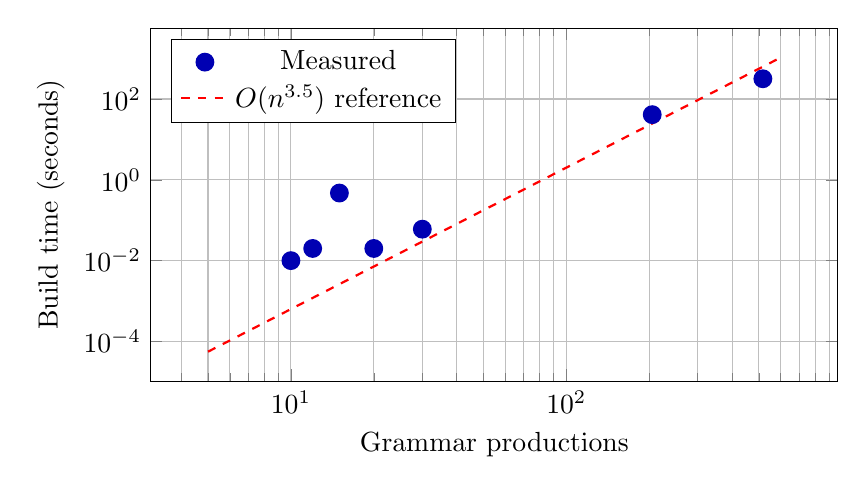
\begin{tikzpicture}
\begin{axis}[
  xlabel={Grammar productions},
  ylabel={Build time (seconds)},
  xmode=log, ymode=log,
  log basis x=10, log basis y=10,
  grid=both,
  width=0.85\textwidth,
  height=0.5\textwidth,
  mark size=3pt,
  legend pos=north west,
]
\addplot[only marks, mark=*, blue!70!black, thick] coordinates {
  (10,  0.01)
  (12,  0.02)
  (15,  0.47)
  (20,  0.02)
  (30,  0.06)
  (205, 40.9)
  (517, 315.7)
};
\addplot[domain=5:600, samples=50, red, dashed, thick]
  {0.0000002 * x^3.5};
\legend{Measured, $O(n^{3.5})$ reference}
\end{axis}
\end{tikzpicture}
\caption{Log-log plot of build time vs.\ production count.
  The two largest grammars (CSP and SV) follow an approximately
  cubic-to-quartic trend.  Small grammars are dominated by startup overhead.
  The \texttt{cmd.y} outlier (15 productions, 0.47\,s) has deeply
  recursive nonterminals that inflate the return-address space.}
\label{fig:scaling}
\end{figure}

The key observation: from CSP (205 productions) to SV (517
productions) is a $2.5\times$ increase in grammar size, but a
$7.7\times$ increase in build time and a $3.8\times$ increase in state
entries.  The scaling is clearly super-linear.

%======================================================================
\section{How \texttt{kyacc} Works}

\subsection{Overview}

\texttt{kyacc} is implemented in $\sim$1,900 lines of Modula-3 across
four key source files, plus supporting libraries.  The compilation
pipeline is:

\begin{enumerate}[nosep]
\item Parse the \texttt{.y} grammar via \texttt{YaccParse}
\item Build the LR automaton via \texttt{PDA.BuildStatesList()}
\item Merge equivalent states via \texttt{PDATransListOp.MergeStates()}
\item Flatten transition lists via \texttt{PDATransListFlat.Flatten()}
\item Generate Modula-3 parser source from code templates
\end{enumerate}

Steps 2--4 dominate the runtime.

\subsection{The Mark-Based Item Representation}

Unlike standard LALR(1) generators, \texttt{kyacc} uses an extended
item representation called a ``mark.''  Each mark contains four
fields:

\begin{lstlisting}[language=Modula2]
Mark.T = RECORD
  current: Pos.T;    (* position of dot in a grammar rule *)
  return:  Pos.T;    (* return address: where to continue after reduce *)
  first:   Rule.T;   (* first rule reduced to reach this mark *)
  baseRule: Rule.T;  (* rule for precedence comparison *)
END;
\end{lstlisting}

The critical difference from standard LR items is the \texttt{return}
field.  In a standard LALR(1) generator, two items with the same LR(0)
core (same rule and dot position) are \emph{merged} into a single
state, differing only in their lookahead sets.  In \texttt{kyacc},
items with different \texttt{return} positions are \emph{distinct
marks}, and states containing different mark sets are never merged.

This gives \texttt{kyacc} the power of a canonical LR(1) parser (or
something close to it), but with the corresponding state explosion.

\subsection{State Construction: \texttt{BuildStatesList}}

The automaton is built by BFS exploration
(\texttt{PDA.m3} lines 109--176):

\begin{lstlisting}[language=Modula2,escapechar=@]
REPEAT
  cur := ReverseD(boundary);
  boundary := NIL;
  REPEAT
    curState := cur.head;
    FOR i := 0 TO LAST(self.codes^) DO        @\textrm{\color{red}$\leftarrow$ all symbols}@
      code := self.codes[i];
      action := Step(curState, code, ...);     @\textrm{\color{red}$\leftarrow$ scans all marks}@
      CASE action.kind OF
      | Shift =>
        Expand(action.next, ...);              @\textrm{\color{red}$\leftarrow$ rebuild closure}@
        curTrans.target := GetState(action.next);
      ...
    END;
  UNTIL cur = NIL;
UNTIL boundary = NIL;
\end{lstlisting}

For each state, the algorithm iterates over \emph{every} symbol code
and calls \texttt{Step()}, which scans the entire mark list.  For
shifts, it calls \texttt{Expand()} to compute the epsilon closure of
the new state.

\subsection{Epsilon Closure: \texttt{Expand} and \texttt{AddMark}}

\texttt{Expand()} (\texttt{RuleListState.m3} lines 199--209) rebuilds
the mark set from scratch every time it is called:

\begin{lstlisting}[language=Modula2]
PROCEDURE Expand(self: T; VAR est: INTEGER) =
  VAR cur := self.marksList;
  BEGIN
    ClearMarksTable(self, est);      (* delete old hash table *)
    WHILE cur # NIL DO
      AddMark(self, cur.head);       (* re-add each mark *)
      cur := cur.tail;
    END;
    BuildMarksList(self, est);       (* sort marks into list *)
  END Expand;
\end{lstlisting}

\texttt{AddMark()} is recursive---it chases both ``call'' edges
(entering a nonterminal) and ``return'' edges (completing a rule).
For each mark, it looks up all rules that produce the symbol at the
dot position and recursively adds marks for each:

\begin{lstlisting}[language=Modula2,escapechar=@]
PROCEDURE AddMark(self: T; READONLY mark: Mark.T) =
  BEGIN
    IF mark.current.cell = NIL THEN
      (* at end of rule: chase return address *)
      IF mark.return.rule # NIL THEN
        AddMark(self, Mark.T{current := mark.return, ...});  @\textrm{\color{red}$\leftarrow$ recursive}@
      END;
    ELSIF NOT self.marksTab.get(mark, bool) THEN
      EVAL self.marksTab.put(mark, TRUE);
      (* chase all rules for the symbol at dot position *)
      EVAL self.call.get(Sym.GetCode(callSym), cur);
      WHILE cur # NIL DO
        AddMark(self, Mark.T{current := Pos.Zero(cur.head),  @\textrm{\color{red}$\leftarrow$ recursive}@
                               return := return, ...});
        cur := cur.tail;
      END;
    END;
  END AddMark;
\end{lstlisting}

There is no memoization.  The same nonterminal's expansion is
recomputed in every state that references it.

\subsection{State Deduplication}

New states are looked up in a hash table
(\texttt{RuleListStateTbl}).  The hash function for a state is:

\begin{lstlisting}[language=Modula2]
PROCEDURE Hash(self: T): INTEGER =
  RETURN Rule.Number(self.finish) + 3 * MarkListF.Hash(self.marksList);
\end{lstlisting}

where \texttt{MarkListF.Hash} traverses the \emph{entire linked list}
of marks, accumulating:

\begin{lstlisting}[language=Modula2]
PROCEDURE Hash(l: T): INTEGER =
  VAR cur := l;  acc: INTEGER := 0;
  BEGIN
    WHILE cur # NIL DO
      acc := acc * 3 + Elem.Hash(cur.head);
      cur := cur.tail;
    END;
    RETURN acc;
  END Hash;
\end{lstlisting}

Each \texttt{Mark.Hash} only uses 2 of its 4 fields
(\texttt{current} and \texttt{return} positions), ignoring
\texttt{first} and \texttt{baseRule}.  This produces more hash
collisions than necessary, causing expensive equality checks.

Equality comparison (\texttt{MarkListF.Equal}) walks both linked
lists element-by-element, comparing each mark field by field.

\subsection{Post-Processing: State Merging and Flattening}

After all states are built, \texttt{MergeStates()} runs a
fixed-point iteration that looks for states with identical transition
lists and merges them:

\begin{lstlisting}[language=Modula2]
REPEAT
  fixed := TRUE;
  canonID := NEW(PDATransListIntTbl.Default).init();
  WHILE i <= newNumStates DO
    IF canonID.get(a[i], ID) THEN
      fixed := FALSE;    (* found duplicate, renumber and retry *)
    ELSE
      EVAL canonID.put(a[i], ID);
    END;
    ...
  END;
  ReNumberShifts();
UNTIL fixed;
\end{lstlisting}

This requires multiple passes because merging two states changes
the transition targets of other states, potentially creating new
merge opportunities.  Each pass is $O(\text{states} \times
\text{transitions})$.

%======================================================================
\section{Root Cause Analysis}

\subsection{The Fundamental Issue: Not LALR(1)}

The single most important factor is that \texttt{kyacc} builds
something close to a \textbf{canonical LR(1)} automaton rather than
LALR(1).  The mark's \texttt{return} field encodes the call context,
so two items that would share an LALR(1) state (same LR(0) core,
different lookaheads) remain in separate states in \texttt{kyacc}.

This is by design---it gives \texttt{kyacc} more power to resolve
conflicts---but it causes the state count to grow much faster than
LALR(1).  For the SV grammar, the generated parser has 68,285 state
entries after flattening, compared to what would likely be 1,000--2,000
LALR(1) states for a grammar of this size.

\subsection{Quadratic Inner Loop}

For each of the $S$ states, the algorithm iterates over all $C$
symbol codes and calls \texttt{Step()}, which scans all $M$ marks:

\[
T_{\text{step}} = O(S \times C \times M)
\]

For the SV grammar: $C = 160$ symbols, but most \texttt{Step()} calls
return \texttt{Error} (no mark has that symbol at its dot position).
The algorithm does not precompute which symbols are relevant to each
state.

\subsection{Redundant Closure Computation}

\texttt{Expand()} is called once per new state discovery, and
rebuilds the epsilon closure from scratch each time.  The closure of a
nonterminal like \texttt{expression}---which appears in 50+ places in
the grammar and recurses through 16 levels of precedence
climbing---is recomputed in every state that references it.

For a grammar with $N$ nonterminals of average depth $D$ and $R$ rules
per nonterminal, each \texttt{Expand()} call performs
$O(M \times D \times R)$ recursive \texttt{AddMark()} calls, where $M$
is the number of seed marks.

\subsection{Expression Hierarchy Depth}

The SV grammar's expression precedence chain is 16 levels deep:

\begin{lstlisting}[language={},basicstyle=\ttfamily\footnotesize]
expression -> cond_expr -> lor_expr -> land_expr -> bor_expr
-> bxor_expr -> band_expr -> eq_expr -> rel_expr -> shift_expr
-> add_expr -> mul_expr -> unary_expr -> pow_expr -> postfix_expr
-> primary_expr
\end{lstlisting}

Every occurrence of \texttt{expression} on a rule's RHS generates
marks at each of these 16 levels, each with a different return
address.  Since \texttt{expression} appears in $\sim$50 contexts, this
creates a combinatorial explosion of marks: each context $\times$ each
precedence level $\times$ each return path.

\subsection{Linked-List Data Structures}

Mark sets are stored as sorted linked lists (\texttt{MarkList.T}).
This means:

\begin{itemize}[nosep]
\item \texttt{Step()}: linear scan to find marks matching a symbol, $O(M)$
\item \texttt{Hash()}: full list traversal, $O(M)$
\item \texttt{Equal()}: element-by-element comparison, $O(M)$
\item No random access, no binary search
\end{itemize}

Combined with the hash table's collision rate (poor 2-field hash on
4-field records), state deduplication is expensive.

\subsection{Complexity Summary}

\begin{table}[h]
\centering
\begin{tabular}{@{}llll@{}}
\toprule
Operation & Location & Complexity & Notes \\
\midrule
State BFS & \texttt{PDA.BuildStatesList} & $O(S \times C \times M)$ &
  $C$ = all symbols, not just relevant \\
Epsilon closure & \texttt{RuleListState.Expand} & $O(M \times D \times R)$ &
  Rebuilt from scratch each time \\
\texttt{AddMark} recursion & \texttt{RuleListState.AddMark} & $O(D \times R)$ &
  No memoization \\
State hashing & \texttt{MarkListF.Hash} & $O(M)$ per state &
  2/4 fields used, poor distribution \\
State equality & \texttt{MarkListF.Equal} & $O(M)$ per comparison &
  Linked-list traversal \\
State merging & \texttt{MergeStates} & $O(I \times S \times T)$ &
  $I$ = fixed-point iterations \\
\bottomrule
\end{tabular}
\caption{Complexity of major operations.  $S$ = states, $C$ = symbol codes,
  $M$ = marks per state, $D$ = nonterminal depth, $R$ = rules per
  nonterminal, $T$ = transitions per state, $I$ = merge iterations.}
\end{table}

The total work is approximately:
\[
T_{\text{total}} \approx S \cdot \bigl( C \cdot M + M \cdot D \cdot R \bigr)
  + I \cdot S \cdot T
\]
where $S$ itself grows super-linearly with grammar size due to
the return-address state explosion.

%======================================================================
\section{Proposed Fixes}

We identify eight potential optimizations, divided into grammar-level
changes (specific to the SV grammar) and generator-level changes
(to \texttt{kyacc} itself).

\subsection{Grammar-Level Fixes}

\subsubsection{G1: Flatten the Expression Precedence Chain}

\textbf{Impact: high. \quad Effort: moderate.}

The 16-level expression hierarchy is the single largest contributor to
mark-set inflation.  Every occurrence of \texttt{expression} on a
RHS creates return-address marks at all 16 levels.  Collapsing the
chain to 5--6 levels by grouping operators at similar precedence would
dramatically reduce state counts.

For example, the four levels \texttt{bor\_expr}, \texttt{bxor\_expr},
\texttt{band\_expr}, and \texttt{eq\_expr} could be merged into a
single \texttt{bitwise\_expr} nonterminal with explicit rule-level
precedence resolution (which \texttt{kyacc} already supports via
\texttt{Rule.Compare}).

\textbf{Expected improvement:} 3--5$\times$ reduction in state count.

\subsubsection{G2: Factor Common Prefixes in Port Declarations}

\textbf{Impact: moderate. \quad Effort: moderate.}

\texttt{port\_decl} has 31 alternatives, many sharing the prefix
\texttt{port\_direction} followed by a type keyword.  Refactoring into:

\begin{lstlisting}[language={}]
port_decl:
  directed          port_direction port_decl_body
  undirected        port_decl_undirected
  connection        port_connection
\end{lstlisting}

would allow the parser to share states across the common prefix
rather than maintaining separate state chains for each alternative.

Similarly, \texttt{param\_port\_decl} (13 alternatives) and
\texttt{statement} (27 alternatives) would benefit from factoring.

\textbf{Expected improvement:} 1.5--2$\times$ reduction in state count.

\subsubsection{G3: Inline Small Optional Nonterminals}

\textbf{Impact: moderate. \quad Effort: low.}

Nonterminals like \texttt{opt\_signing} (3 alternatives),
\texttt{opt\_packed\_dims} (2 alternatives), and
\texttt{opt\_unpacked\_dims} (2 alternatives) are referenced from
15+ places each.  Each reference creates return-address variants in the
mark set.

Inlining these---duplicating the parent rule's alternatives for each
option---eliminates one level of nonterminal indirection per reference.
The grammar becomes more verbose, but the mark sets shrink.

\textbf{Expected improvement:} 1.5--2$\times$ reduction in state count,
concentrated in the declaration-heavy parts of the grammar.

\subsection{Generator-Level Fixes}

\subsubsection{K1: Iterate Only Relevant Symbols per State}

\textbf{Impact: high. \quad Effort: low.}

The inner loop in \texttt{BuildStatesList} iterates over all 160+
symbol codes for every state.  Most calls to \texttt{Step()} return
\texttt{Error} because the symbol doesn't appear at any dot position
in the current state.

Fix: before the symbol loop, collect the set of symbols that appear at
dot positions in the current state's marks.  This is a single pass
over the mark list:

\begin{lstlisting}[language=Modula2]
(* Collect relevant symbols *)
relevant := NEW(IntBoolTbl.Default).init();
cur := curState.marksList;
WHILE cur # NIL DO
  EVAL relevant.put(Sym.GetCode(cur.head.current.cell.head), TRUE);
  cur := cur.tail;
END;
(* Iterate only relevant symbols *)
iter := relevant.iterate();
WHILE iter.next(code, dummy) DO
  action := Step(curState, code, ...);
  ...
END;
\end{lstlisting}

A typical state has transitions on 5--15 symbols.  This reduces the
inner loop from 160 iterations to $\sim$10.  \textbf{Note:}
implementation and testing (Section~7) showed only a 13\% improvement,
indicating \texttt{Step()} is not the dominant cost---\texttt{Expand()}
is the true bottleneck.

\subsubsection{K2: Memoize Epsilon Closures}

\textbf{Impact: high. \quad Effort: moderate.}

The epsilon closure of a nonterminal (the set of marks reachable by
following call edges from a given starting position) is deterministic
given the starting mark.  Currently, \texttt{Expand()} recomputes it
from scratch for every state.

A cache keyed on the set of seed marks (the marks before closure
expansion) would allow reuse.  For a grammar like SV where the same
nonterminal (\texttt{expression}, \texttt{statement}, etc.)\ is
entered from thousands of states, this would eliminate most
\texttt{AddMark()} recursion.

\textbf{Expected improvement:} 5--10$\times$ on \texttt{Expand()} cost.

\subsubsection{K3: Switch to LALR(1) Core Merging}

\textbf{Impact: transformative. \quad Effort: high.}

The fundamental fix is to separate the LR(0) core from the
context/lookahead information in each mark, and merge states that share
the same core.  This is the approach used by yacc, Bison, and
essentially all practical parser generators.

The mark representation would become:

\begin{lstlisting}[language=Modula2]
CoreItem = RECORD
  rule: Rule.T;
  index: INTEGER;     (* dot position *)
END;

ContextItem = RECORD
  core: CoreItem;
  lookahead: SET OF Symbol;  (* or return address set *)
END;
\end{lstlisting}

States would be keyed only by their set of core items.  Conflicts
that the current return-address mechanism resolves would need to be
handled by the standard LALR(1) lookahead propagation algorithm
(DeRemer and Pennello, 1982).

This would reduce the SV grammar's state count from $\sim$68,000
entries to an estimated 1,000--2,000, and build time from 5 minutes to
well under one second.

\textbf{Expected improvement:} 100--1000$\times$.  But requires a
significant rewrite of \texttt{RuleListState}, \texttt{PDA}, and
the conflict resolution logic.

\subsubsection{K4: Improve the Hash Function}

\textbf{Impact: moderate. \quad Effort: low.}

The current \texttt{Mark.Hash} uses only 2 of 4 fields:

\begin{lstlisting}[language=Modula2]
PROCEDURE Hash(a: T): INTEGER =
  RETURN Pos.Hash(a.current) + Pos.Hash(a.return) * 17;
\end{lstlisting}

Including \texttt{first} and \texttt{baseRule} would reduce collisions
in the state deduplication table:

\begin{lstlisting}[language=Modula2]
PROCEDURE Hash(a: T): INTEGER =
  RETURN Pos.Hash(a.current) + Pos.Hash(a.return) * 17
       + Rule.Number(a.first) * 31 + Rule.Number(a.baseRule) * 7;
\end{lstlisting}

\textbf{Expected improvement:} 1.5--2$\times$ on state deduplication.

\subsubsection{K5: Use Arrays Instead of Linked Lists for Mark Sets}

\textbf{Impact: moderate. \quad Effort: moderate.}

Replacing \texttt{MarkList.T} (singly-linked list) with a sorted
array would enable:

\begin{itemize}[nosep]
\item Binary search in \texttt{Step()}: $O(\log M)$ instead of $O(M)$
\item Faster \texttt{Hash()}: contiguous memory, no pointer chasing
\item Faster \texttt{Equal()}: \texttt{memcmp}-style comparison with
  early termination
\item Precomputed hash values stored with the array
\end{itemize}

\textbf{Expected improvement:} 2--3$\times$ on mark-set operations.

%======================================================================
\section{Recommended Action Plan}

Fixes are ranked by effort-to-impact ratio:

\begin{table}[h]
\centering
\begin{tabular}{@{}clccl@{}}
\toprule
Priority & Fix & Impact & Effort & Speedup \\
\midrule
1 & K1: Relevant symbols only & Low    & Low      & 1.13$\times$ \emph{(measured)} \\
2 & G1: Flatten expressions   & High   & Moderate & 3--5$\times$ \\
3 & K4: Better hash function  & Moderate & Low    & 1.5--2$\times$ \\
4 & K2: Memoize closures      & High   & Moderate & 5--10$\times$ \\
5 & G3: Inline optionals      & Moderate & Low    & 1.5--2$\times$ \\
6 & G2: Factor prefixes       & Moderate & Moderate & 1.5--2$\times$ \\
7 & K5: Array mark sets       & Moderate & Moderate & 2--3$\times$ \\
8 & K3: LALR(1) rewrite       & Transformative & High & 100--1000$\times$ \\
\bottomrule
\end{tabular}
\caption{Proposed fixes ranked by effort-to-impact ratio.
  Fixes K1 + G1 + K4 together would likely reduce build time
  from 5 minutes to 5--15 seconds.  Fix K3 alone would reduce it
  to well under 1 second, but requires a major rewrite.}
\label{tab:fixes}
\end{table}

K1 (relevant symbols only) has been implemented and delivers a
measured 13\% improvement (see Section~7).  This confirms that the
\texttt{Step()} symbol loop is \emph{not} the dominant cost.

The pragmatic path forward is K2 (memoize epsilon closures),
targeting the confirmed bottleneck in \texttt{Expand()}/\texttt{AddMark()}.
Combined with grammar refactoring (G1, flatten expression hierarchy),
these should bring the SV grammar build time down to a tolerable
range of 10--30 seconds.

The ideal long-term fix remains K3 (LALR(1) core merging), which would
make grammar size essentially irrelevant to build performance.
However, this requires understanding the trade-offs: \texttt{kyacc}'s
current return-address mechanism may resolve certain conflicts that
LALR(1) cannot, and those cases would need alternative handling.

%======================================================================
\section{Experimental Results: K1 Implementation}

We implemented optimization K1 (relevant symbols only) and tested it
on the SV grammar.  The implementation adds two new procedures to
\texttt{RuleListState}:

\begin{lstlisting}[language=Modula2]
PROCEDURE CollectRelevantCodes(self: T;
                               relevant: REF ARRAY OF BOOLEAN);
(* Set relevant[code] := TRUE for each symbol code
   at a dot position in self's mark list *)

PROCEDURE QuickAction(self: T; code: INTEGER): Action;
(* Fast action for a code NOT at any dot position.
   Returns Reduce(finish), Accept, or Error. *)
\end{lstlisting}

In \texttt{PDA.BuildStatesList}, a boolean array indexed by symbol code
is allocated once outside the main loop.  Before the per-symbol
iteration in each state, the array is cleared and populated by
\texttt{CollectRelevantCodes}.  The inner loop then dispatches:

\begin{lstlisting}[language=Modula2]
FOR i := 0 TO LAST(self.codes^) DO
  code := self.codes[i];
  IF relevant[code] THEN
    action := Step(curState, code, self.symNames[code]);
  ELSE
    action := QuickAction(curState, code);
  END;
  ...
END;
\end{lstlisting}

\texttt{QuickAction} avoids scanning the mark list entirely---it
checks only the \texttt{start} status and the \texttt{finish} field
(for default reductions) plus a single hash table lookup in the
\texttt{call} table.

\subsection{Results}

\begin{center}
\begin{tabular}{@{}lrrl@{}}
\toprule
Configuration & Wall time & User time & Speedup \\
\midrule
Baseline (original kyacc)  & 5m 16s & 5m 12s & --- \\
With K1 optimization       & 4m 36s & 4m 33s & 13\% \\
\bottomrule
\end{tabular}
\end{center}

Output was verified identical (diff of generated parser interfaces
showed only the expected name difference).

\subsection{Analysis: Why Only 13\%?}

The 13\% improvement---far short of the predicted 10--20$\times$---reveals
that \textbf{\texttt{Step()} is not the dominant cost}.  The per-symbol
loop accounts for only $\sim$15\% of total runtime.

The true bottleneck is \texttt{Expand()}/\texttt{AddMark()}, which
rebuilds the epsilon closure for every new state.  For the SV grammar,
with its 16-level expression hierarchy and $\sim$50 contexts referencing
\texttt{expression}, each \texttt{Expand()} call triggers thousands
of recursive \texttt{AddMark()} invocations chasing call and return
edges through the grammar.  This work is repeated identically in
every state that references the same nonterminals.

This shifts the priority ranking:

\begin{itemize}[nosep]
\item \textbf{K2 (memoize closures)} is now the highest-impact
  generator-level fix, targeting the actual bottleneck
\item \textbf{G1 (flatten expressions)} remains high-impact, as it
  reduces the recursion depth that makes \texttt{Expand()} expensive
\item \textbf{K1 is still worth keeping}---it eliminates unnecessary
  work and its 13\% gain is free
\end{itemize}

\subsection{Revised Priority Table}

\begin{table}[h]
\centering
\begin{tabular}{@{}clccl@{}}
\toprule
Priority & Fix & Impact & Effort & Speedup \\
\midrule
1 & K2: Memoize closures      & High   & Moderate & 5--10$\times$ (est.) \\
2 & G1: Flatten expressions   & High   & Moderate & 3--5$\times$ (est.) \\
3 & K4: Better hash function  & Moderate & Low    & 1.5--2$\times$ (est.) \\
4 & K1: Relevant symbols only & Low    & Low      & \textbf{1.13$\times$ (measured)} \\
5 & G3: Inline optionals      & Moderate & Low    & 1.5--2$\times$ (est.) \\
6 & G2: Factor prefixes       & Moderate & Moderate & 1.5--2$\times$ (est.) \\
7 & K5: Array mark sets       & Moderate & Moderate & 2--3$\times$ (est.) \\
8 & K3: LALR(1) rewrite       & Transformative & High & 100--1000$\times$ (est.) \\
\bottomrule
\end{tabular}
\caption{Revised priorities after K1 implementation.  K2 (memoize
  closures) is now the recommended next step, as \texttt{Expand()} is
  the confirmed bottleneck.  K1's measured 1.13$\times$ replaces the
  original 10--20$\times$ estimate.}
\label{tab:revised-fixes}
\end{table}

%======================================================================
\section{Source File Reference}

\begin{table}[h]
\centering
\begin{tabular}{@{}llrl@{}}
\toprule
File & Path (relative to \texttt{caltech-parser/parserlib/}) & Lines & Role \\
\midrule
\texttt{PDA.m3}             & \texttt{kyacc/src/}    & 308 & State table construction \\
\texttt{RuleListState.m3}   & \texttt{kyacc/src/}    & 381 & Item set closure \\
\texttt{PDATransListOp.m3}  & \texttt{kyacc/src/}    & 172 & State merging \\
\texttt{PDATransListFlat.m3}& \texttt{kyacc/src/}    & 157 & Transition flattening \\
\texttt{Mark.m3}            & \texttt{kyacc/src/}    &  47 & LR item (mark) record \\
\texttt{Pos.m3}             & \texttt{kyacc/src/}    &  65 & Position within rules \\
\texttt{Main.m3}            & \texttt{kyacc/src/}    & 145 & Driver and code generation \\
\texttt{Rule.m3}            & \texttt{kyacclib/src/} &  -- & Grammar rule representation \\
\texttt{Sym.m3}             & \texttt{kyacclib/src/} &  -- & Symbol representation \\
\texttt{YaccParse.m3}       & \texttt{kyacclib/src/} &  -- & Grammar file parser \\
\texttt{ListF.mg}           & \texttt{cit\_util/src/} &  111 & Generic list Hash/Equal \\
\bottomrule
\end{tabular}
\caption{Key source files in \texttt{kyacc} and its libraries.}
\end{table}

\end{document}
